% % % % % % % % %part-15% % % % % % % % %
\documentclass[12pt]{article}

%\usepackage{tikz}
\usepackage{pgfplots}

\author{Chandra Has\\ chandrahashbti@gmail.com}
\title{{\color{red}\bfseries Graphing} in \LaTeX\ using PGF/TikZ}\date{}

\begin{document}\maketitle\vskip-25pt\hrule\vskip10pt\centering

%1. axis range: [xmin, xmax, ymin, ymax]
%2. domain: sampling interval in the form of a:b
%3. Samples: samples=N, samples at={x1,x2,x3,...}, no. of samlples inserted into the sampling interval

%Expressions:
%1. polynomial
%2. trigonometric
%3. exponential
%4. logarithmic

\begin{tikzpicture}
\begin{axis}[xmin=0, xmax=5, ymin=0, ymax=5, width=7cm, height=7cm, xtick distance=1.2, ytick distance=1.2]

\end{axis}
\end{tikzpicture}

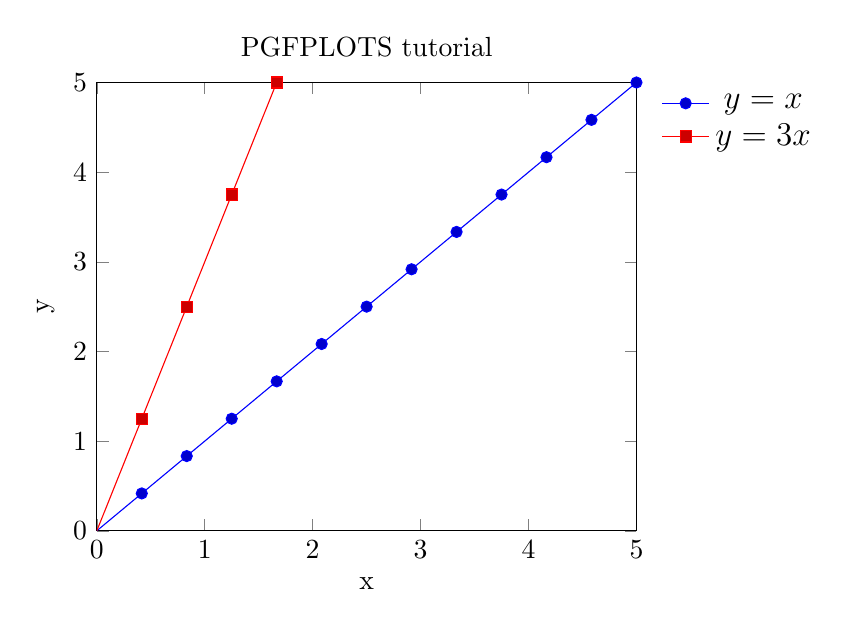
\begin{tikzpicture}
\begin{axis}[xmin=0, xmax=5, ymin=0, ymax=5, xlabel=x, ylabel=y, title=PGFPLOTS tutorial, legend entries={$y=x$, $y=3x$}, legend style={font=\large, draw=none, legend pos=outer north east} ]
\addplot  {x};
\addplot  {3*x};
\end{axis}
\end{tikzpicture}


%Legend
%legend entries={<legend 1, legend 2, legend 3,...>}
%legend style={<key-value-list>},
%styles for legend---> draw=none, shape=<shape name>, at={(point)}, legend columns=<num>, legend cell align=<left|center|right>, legend pos={<north east, outer north east, south east, north west, south west, ...>},

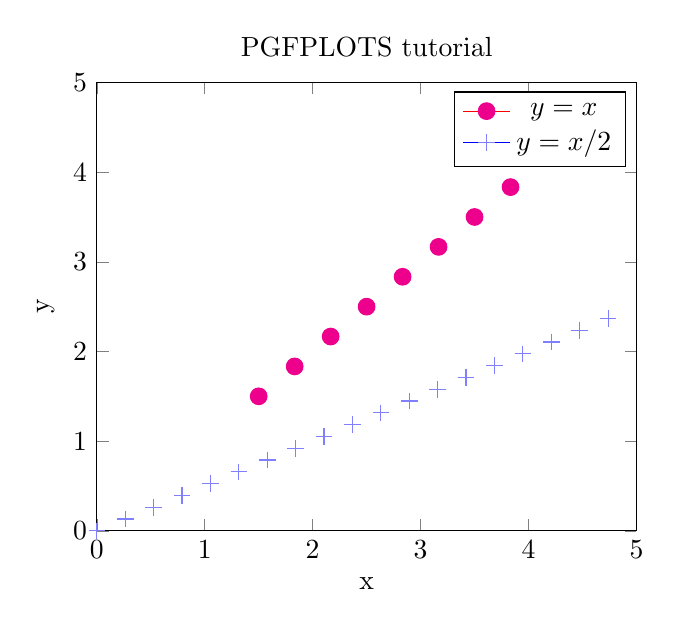
\begin{tikzpicture}
\begin{axis}[xmin=0, xmax=5, ymin=0, ymax=5, xlabel=x, ylabel=y, title=PGFPLOTS tutorial, legend entries={$y=x$, $y=x/2$} ]
\addplot[draw=none, domain=1.5:4.5, mark=*, samples=10, red, mark options={magenta, mark size=3pt}]  {x};
\addplot[draw=none, domain=0:5, samples=20, mark=+, blue, mark options={blue!50, mark size=3pt}]  {x/2};
\end{axis}
\end{tikzpicture}

%Plot options:
%The axis- and the plot-options are largely the same: it is just that the plot-options override corresponding attributes set in the axis-options.
%
%color name, thickness, dashed, solid, dotted, dashdotted, dashdotdotted, samples=<num>, samples at = {x values separated by comma}, domain=m:n, draw, draw=none, mark=<symbol (e.g., ball, +,*, -, x,)>, no markers, only marks, mark size=<dimension>, mark options={<key-value-list, e.g., color=red, rotate=45>},  mark repeat=n, nodes near coords, smooth, sharp plot, variable=<name> 

\begin{tikzpicture}
\begin{axis}[xmin=0, xmax=5, ymin=0, ymax=5, xlabel=x, ylabel=y, title=PGFPLOTS tutorial, legend entries={$y=x$} ]
\addplot[draw=none, domain=1.5:4.5, mark=*, samples at ={1.5, 3, 4, 4.5}, red]  {x};
\end{axis}
\end{tikzpicture}

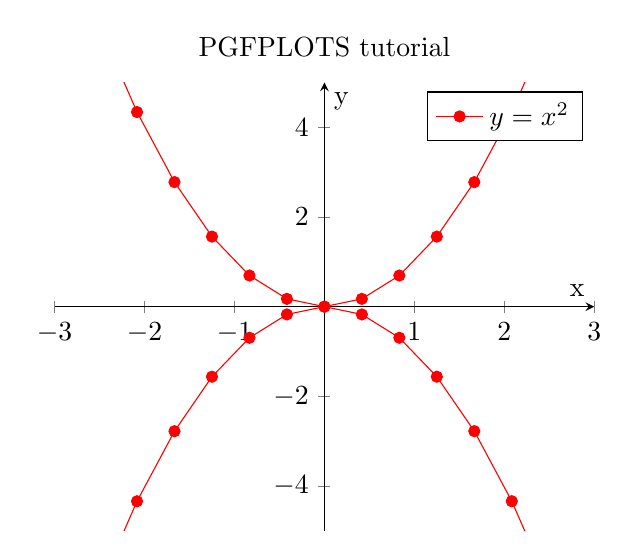
\begin{tikzpicture}
\begin{axis}[xmin=-3, xmax=3, ymin=-5, ymax=5, xlabel=x, ylabel=y, title=PGFPLOTS tutorial, legend entries={$y=x^2$}, axis lines=center ]
\addplot[mark=*, red]  {x^2};
\addplot[mark=*, red]  {-x^2};
\end{axis}
\end{tikzpicture}

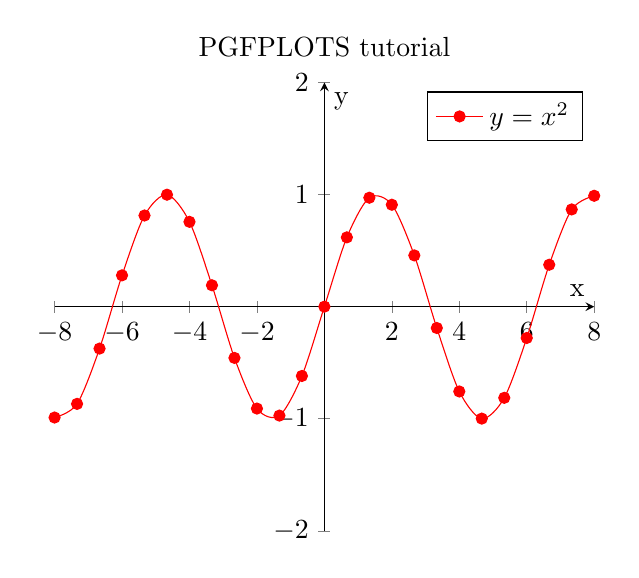
\begin{tikzpicture}
\begin{axis}[xmin=-8, xmax=8, ymin=-2, ymax=2, xlabel=x, ylabel=y, title=PGFPLOTS tutorial, legend entries={$y=x^2$}, axis lines=center ]
\addplot[mark=*, red, domain=-8:8, smooth]  {sin(deg (x))};
\end{axis}
\end{tikzpicture}

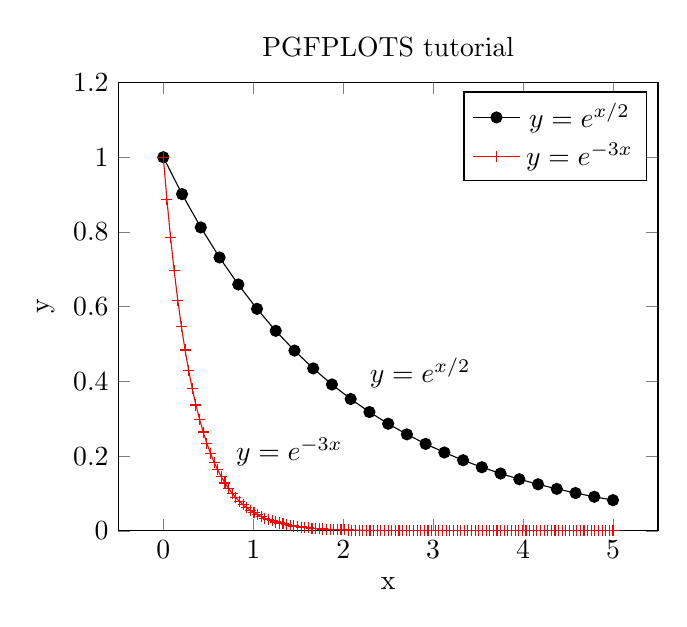
\begin{tikzpicture}
\begin{axis}[ymin=0, ymax=1.2, xlabel=x, ylabel=y, title=PGFPLOTS tutorial, legend entries={$y=e^{x/2}$, $y= e^{-3x}$}]
\addplot[mark=*, domain=0:5]  {exp(-x/2)};
\addplot+[mark=+, domain=0:5, samples=125]  {exp(-3*x)};
\node[above=2cm, right=2.5cm] {$y=e^{x/2}$};
\node[above=1cm, right=0.8cm] {$y= e^{-3x}$};
\end{axis}
\end{tikzpicture}



\end{document}












